\section{Implementation and Experiments}

\subsection{Clause Reduction with $\IUIP$}
To evaluate $\IUIP$'s effectiveness as a clause reduction technique, we implement  $\IUIPPURE$ and $\IUIPMIN$  on top of \text{\MapleBase} \cite{}, the winner of SAT Race 2015 application track.  We than compare the performance of the baseline $\MapleBase$ with $\MapleIUIPPURE$ and $\MapleIUIMIN$ on the full set of benchmarks from SAT RACE 2019 main track.

The benchmark contains 400 instances divided into two groups of 200, new and old, representing historical instances and fresh instances in the 2019 race, respectively. I partition the old group instances into six partitions of size 30 and one partition of size 20. Each partition is then assigned to a Intel CPU node with 16 cores (2 sockets 8 cores  and  1 thread) and 96649 MB memory. The new group is partitioned based on their contributor (e.g. Heule contributed 22 matrix multiplication instances), and each partition is assigned to a aforementioned CPU node. To speed up the experiment, we allow a CPU node to solver at most seven instances concurrently. 

Beside solved instances and PAR-2 score, we additionally measure the average clause length and clause reduction ratio for each instances. For $\MapleIUIPPURE$  and $\MapleIUIMIN$, we also captures the $\IUIP$ learning attempted rate and success rate.

\nf{Inserted a table here, and graphs and analysis}




\begin{center}
\begin{tabular}{ | m{3.5cm} | m{2cm}| m{2cm} | m{2cm} | m{2.5cm} | } 
\hline
Solver & \# solved & PAR-2 & Clause Size & Cl Reduction\% \\ 
\hline
$\MapleBase$ & 221 & 5005.2 & 62.6 & 36.53\% \\ 
\hline
$\MapleIUIPPURE$ & cell9 & cell9 & cell10 & cell11\\ 
\hline
$\MapleIUIMIN$ & 226 & 4933.6 & 45.2 & 47.5\%\\ 
\hline
\end{tabular}
\end{center}


\begin{figure}
    \centering
    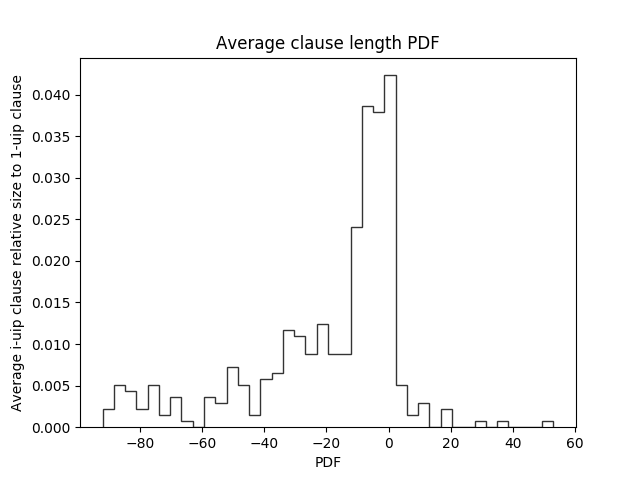
\includegraphics[width=0.8\textwidth, natwidth=610,natheight=642]{clause_length_PDF.png}
    \caption{Average clause (relative to 1-UIP clauses) size distribution. X axis indicates the relative size difference, and Y axis indicates the PDF.}
     \label{fig:len_pdf}
\end{figure}
\begin{figure} \label{fig:len_compare}
    \centering
    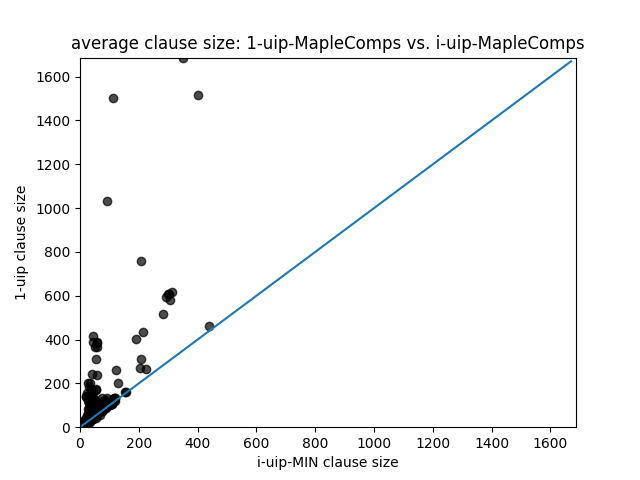
\includegraphics[width=0.8\textwidth, natwidth=610,natheight=642 ]{i-uip-sizes-compare.png}
    \caption{Average clause size comparison plot. Each point in the plot represents an benchmark instance. X and Y axis shows the clause length from $\MapleIUIMIN$ and $\MapleBase$, respectively  }
    \label{fig:len_compare}
\end{figure}





A solver produce smaller clauses can construct smaller proofs as well. For UNSAT instances, we additionally measure their DRUP\cite{} proof checking time as well as the size of the optimized DRUP proof. We used DART-trim \cite{} with 5000 timeout to check and optimize DRUP proofs. 

\nf{Insert a comparison graphs here. (X and Y comparisons graph, showing both time and optimized proof size).}


\subsection{$\IUIP$ as a Practical Learning Scheme}
To evaluate $\IUIP$'s effectiveness as a clause learning scheme, we implement $\IUIPMIN$ on $\MapleBase$ with the extensions mentioned in section~\ref{sec:i-uip}. We evaluated four different configurations (i-UIP, i-UIP-Greedy, i-UIP-Inclusive, and i-UIP-Exclusive) of $\IUIP$ and 1-UIP learning on the SAT Race 2019 main track benchmark and report each configuration's solved instances and PAR-2 score. 

\nf{Inserted a table here, and graphs and analysis}


\subsection{$\IUIP$ on Modern SAT solvers}
To validate $\IUIP$ as a generalizable learning scheme on modern SAT solvers, we re-implement $\IUIP$ on $\MapleSeven$ \cite{},  $\MapleNine$ \cite{} and $\expSAT$.  
The first two solvers are the winner of 2017 and 2019 SAT race, respectively.  $\expSAT$ is a top ten solver from 2019 SAT race which uses random walk simulation to help branch. For each solver, we compare the base 1-UIP learning scheme against top two $\IUIP$ configurations, $\IUIPGreedy$ and $\IUIPActive$, on the SAT Race 2019 main track benchmark. We report solved instances and PAR-2 score.

\nf{Inserted a table here, and graphs and analysis}
